\chapter{Analysis}

\section{Sequencing rhythms}

A traditional electronic \textit{sequencer} is a recording and playback system, which can send and receive the control and performance data needed to regenerate a series of musical events\cite{roads}. This data is in the form of MIDI (Musical Instrument Digital Interface) or more recently OSC (Open Sound Control) messages. The data is sent to audio modules (hardware or software), which do the actual playback of audio. A typical setup for creating music with a sequencer is seen in \cref{fig:sequencer_desc}. Sequencers exists in both hardware and software implementations.

\begin{figure}[H]
    \centering
    
\includegraphics[width=\textwidth]{graphics/sequencer_desc.pdf}
    \caption{A typical setup for creating music with a sequencer}
    \label{fig:sequencer_desc}
\end{figure}

\subsection{Perception of rhythm}
\label{sec:perception}
A general definition of rhythm is given in Oxford Learner's Dictionaries:

\begin{displayquote}
    \textbf{Rhythm} - A strong, regular repeated pattern of movement or sound.
\end{displayquote}

In this project the definition boils down to a sequence of rhythmic events: \textit{onsets} and \textit{rests}, with each possible onset/rest being a \textit{step}. 

For the implementation of a sequencer it is important to consider the human perception of rhythm, and especially our sensitivity to timing, as this determines the time resolution needed.\\
It was observed in 1971, that the \textit{Temporal Auditory Acuity}, our ability to separate audible events, extends down to 1 ms.\cite{green} i.e. if the spacing between two events is below this threshold, we perceive the events as a single event. However this doesn't solely determine the human sensitivity to timing, as this is also a matter of how we perceive changes in periodicity, which according to \cite{roads}[p. 140] extends down to microseconds.\\
This is explained in the cognitive processes of expecting the onset to happen, a specific \textit{metrical expectation}\cite{psychologyofmusic}. This is often associated with listening to repeated patterns with equidistant timing, as this gives rise to an internal clock to which the rhythmic timing can be compared.\cite{parncutt}. Thus, the human timing sensitivity is very case dependent, and a huge research area within cognitive hearing science. For the determination of timing requirements in this project, it is therefore relevant to turn to an industrial design approach.\\
In an interview with \textit{Attack magazine}, the industrial designer Roger Linn, who is famous for engineering the popular \textit{MPC} from \textit{Akai Instruments}, argues that a timing resolution of 96 parts per quarter note, is far enough for sequencing rhythms\cite{linn}, as most grooves grooves can be represented in this resolution. This equals a precision of $\SI{5}{\milli\second}$ at 120 BPM. 


\section{Euclidean rhythms}

% Music generated by a system
% planned vs. generated
% the composers role: planner, programmer 
% programming music as opposed to playing it
    % elaborate on music performed on synthesizers, and algorithmic music - then quote. 
    
\subsection{Euclidean algorithm}
\label{sec:euclidean_ago}
% CMN common music notation 
The euclidean algorithm is a step-by-step procedure that computes the greatest common divisor (GCD) between two integers. 
It is build upon the principle that replacing the larger integer with its difference with the smaller, will not change the GCD. Thus repeating this process will eventually result in two equal numbers, being the GCD. When one of the integers is a prime, the GCD is 1. \\ 

An application of the algorithm for musical purposes is found in the \textit{Euclidean rhythms}, discovered by Godfried Toussaint in 2004, and described in his paper "The Euclidean Algorithm  Generates Traditional Musical Rhythms".\\
From studying a large range of traditional musical rhythms, and especially those of Sub-Saharan African music, Toussaint found an important property: \textquote{their onset patterns are distributed as evenly as possible.}\cite{Toussaint2005TheEA}. Thus, for the purpose of generating these rhythms, the goal is to maximize evenness of pulses, a chain of events, roughly equally spaced in time in a given rhythmic pattern.\cite{parncutt}
This process shows to be close related to the calculation of GCD.\\ 
Euclidean rhythms are represented by 2 parameters, \textit{steps} and \textit{pulses}. The corresponding euclidean rhythm is denoted $E(\text{pulses}, \text{steps})$

For a given number of $n$ steps, and another $k<n$ pulses (onsets), there is $k-n$ rests, which are to be placed as evenly as possible between the pulses, to maximize evenness. 
When $n$ and $k$ have a GCD $g \neq 1$ the result decomposes into exactly $g$ equal sequences of length $\frac{n}{g}$. Otherwise, when $g = 1$ the result will be tailed by one unique sequence.\\
The concept of maximizing evenness of patterns appears in many other applications including stringology (computer science) and SNS accelerators (nuclear physics)\cite{Toussaint2005TheEA}.
E. Bjorklund has proposed an algorithm to solve the problem in a general way\cite{bjorklund}\cite{Demaine2009TheDG}. This algorithm will is explained in the following section. 

\subsection{Bjorklund's algorithm}
\label{sec:bjorklund}
This section explains the algorithm proposed by Bjorklund for SNS timing systems, which calculates the binary sequence that maximizes evenness, given $n$ and $k$. (see \cref{sec:sequencer}) The following description explains the algorithm applied to the problem of euclidean rhythms.\\
% Bjorklund shows that the algorithm finishes in $\mathbb{O}(n)$. \cite{bjorklund} 
For $n$ steps and $k$ pulses, there is $n-k$ rests. Rests and pulses are denoted as 0's and 1's in a binary sequence that represents the rhythmic pattern.\\
The first step is to initialize the binary sequence as pulses followed by rests, which we regard as $k$ sequences with a remainder of $n-k$.   
Each step in the algorithm reduces the number of sequences, with exactly $\text{sequences}-\text{remainder}$, and the resemblance with the euclidean algorithm becomes clear.
We now explain the algorithm step-by-step, with the specific case $n=8$ steps and $k=5$ pulses, thus $8-5 = 3$ rests.\\

Initialization of the binary sequence:

\begin{equation*}
[1][1][1][1][1][0][0][0] \hspace{0.1\textwidth} (3,5)
\end{equation*}

Place 0's after each one, from left to right, giving a new remainder of 2. 

\begin{equation*}
    [10][10][10][1][1] \hspace{0.07\textwidth} (3,2)
\end{equation*}

Move the 1's (remainder sequences) by placing them after each $[10]$ sequence. 

\begin{equation*}
    [101][101][10] \hspace{0.095\textwidth} (2,1)
\end{equation*}

When the number of remainder sequences is 1 or 0, Bjorklund's stopping criteria is met. He argues that, even though we could proceed one step further by placing $[10]$ after the first [101], it doesn't matter as the sequence is cyclic. The two sequences will be a rotation of the same binary sequence, a feature that Toussaint calls \textquote{belonging to the same \textit{Rhythmic Necklace}}\cite{Toussaint2005TheEA}.

\subsection{Representation and polyrhythmic}
\label{sec:polyrhythmic}
The resemblance between binary sequences belonging to the same rhythmic necklace, can be difficult to see from the binary representation used above. Instead, euclidean rhythms are often illustrated in a cyclic representation as seen in \cref{fig:euclid_rot}\cite{Toussaint2005TheEA}. The cyclic representation is created in the following way: A circle perimeter is divided into $n$ pieces, and a polygon connecting the $k$ pulses, represents the rhythm. The rhythm starts in the step labelled '0', and proceeds in clockwise direction.
%  at a given \textsc{Step Time}\tdr{?}

\begin{figure}[H]
    \centering
    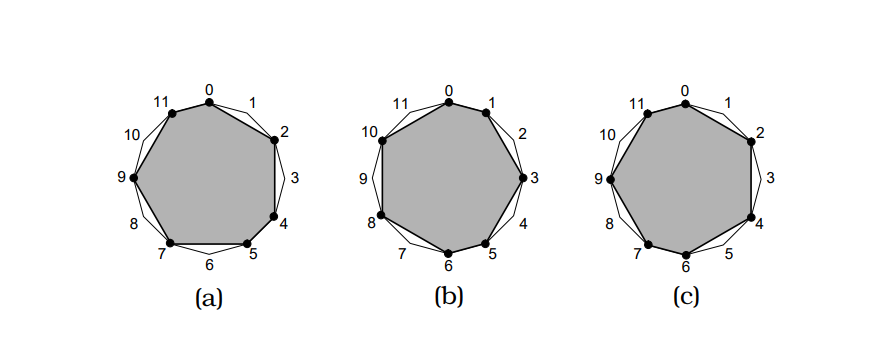
\includegraphics[width=\textwidth]{graphics/euclid_rotation}
    \caption{Illustration taken from \cite{Toussaint2005TheEA}. "Two right-rotations of the Bemb´e string: (a) the Bemb´e, (b) rotation by one unit, (c) rotation by
seven units"}
    \label{fig:euclid_rot}
\end{figure}

This illustration labels a rhythmic identity with a corresponding unique polygon, which might ease the overview and recognition of different euclidean rhythms, as opposed to the binary representation.

When multiple euclidean rhythms are played simultaneously with the same duration between each step (\textit{step time}), it has the interesting possibility of generating polymetric patterns. Polymeter is the concept of instruments playing different meters on top of each other, and thereby desynchronizing themselves. For the case of euclidean rhythms, this happens when the number of steps is different causing the rhythms to have different lengths. \\ 
This is not to be confused with polyrhythms, which, as opposed to polymeters, divides a bar into equal subdivisions, introducing tuplets (duplets, triplets etc.). For euclidean rhythms this would correspond to changing the step time, to make the rhythms have equal lengths.\\ 
A basic difference between the 2 concepts is: polymetric rhythms is locked to a grid but out of phase due to different lengths. Whereas polyrythms are freed from the grid, but all rhythms have equal lengths. This is illustrated in \cref{fig:poly}.

\begin{figure}[H]
    \centering
    \begin{tabular}{lc}
    Ex. 1 & 
    \raisebox{-.5\totalheight}{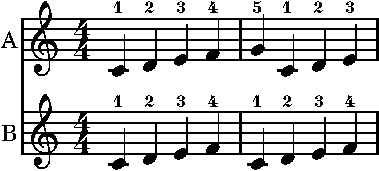
\includegraphics[width=0.5\textwidth]{graphics/polymetric.pdf}}  
    \\ & \\
    Ex. 2 &
    \raisebox{-.5\totalheight}{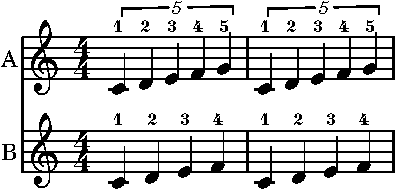
\includegraphics[width=0.5\textwidth]{graphics/polyrhythmic.pdf}}
    \end{tabular}
    \caption{Ex. 1 shows a 5/4 over 4/4 polymetric rhythm. Ex. 2 shows the 5/4 polyrhythm on top of a standard 4/4}
    \label{fig:poly}
\end{figure}

When proceeding after the two bars of polymeters illustrated \cref{fig:poly}, it becomes clear that every bar is different from the former, and that the 5th. bar will be equal to the first, as the patterns resynchronize. Thus, creating and illustrating polymeters in musical notation is somewhat complicated, when compared to euclidean rhythms and their cyclic representation.

% % \begin{displayquote}
% %     CMN was designed to to enable human performance, but when CMN is pushed beyond the limits of human legibility or playability, it no longer serves this function.
% % \end{displayquote}\cite{roads}[p.144]

% Polyrhytmus
In conclusion, the framework of euclidean rhythms is an efficient tool for generating interesting polymetric patterns from traditional rhythms. However, it has 2 significant limitations: 
\begin{itemize}
    \item Due to the nature of the algorithm, the onset-density is constant, making it unsuited for rhythms with fills.
    \item The position of onsets are discrete, making expressive timing (rhythmic variations on micro level) unfeasible.
\end{itemize}

\subsection{Accentuation}
\label{sec:accent}
An important basic feature of rhythmic patterns, which has not been introduced by the framework described above, is dynamic accentuation - the concept of emphasizing certain events by means of a louder sound.\\ 
This allows for rhythms to have a dynamic feel, and a stronger feeling of periodicity. As Peter Q. Pfordresher concludes in his paper, which investigates the perception of melodic and rhythmic accents:
\begin{displayquote}
    Accents function as temporal landmarks that listeners can use when tracking the time structure of musical patterns.
\end{displayquote}\cite{accent}

This cognitive feature of accentuation is especially interesting in combination with euclidean rhythms, when polymetric patterns are generated. Even though the different meters desynchronize, the accents of a static repeating pattern could function as temporal landmarks and thereby give a feeling of periodicity.

\section{Existing sequencers with euclidean rhythms}
\label{sec:existing}
This section contains the survey of 3 existing sequencers that implements euclidean rhythms. The survey is carried out according to the following parameters:
\begin{itemize}
\item Availability for musicians at all technical levels
\item Visual feedback
\item Ease of control
\end{itemize}

\subsubsection{SuperCollider}
Euclidean rhythms are available in the algorithmic composition and audio synthesis tool \textit{SuperCollider} as an extension called \textit{Pbjorklund}. SuperCollider is a programming language and the code for playing the euclidean rhythm $E(5,8)$ is seen in \cref{lst:supercollider}.\\ SuperCollider has very few restrictions and every user can therefore find his/hers own way to use it. However, a disadvantage of SuperCollider is the very limited visual feedback and the requirement of strong programming skills.\\
Control of parameters in SuperCollider is done either by \textit{live coding} (a style of live performance where the performer is programming on stage) or by using a custom MIDI controller setup.

\begin{lstlisting}[caption={Euclidean rhythm $E(5,8)$ in SuperCollider}, label={lst:supercollider}]
Pbind(\dur, Pbjorklund2(5, 8)).play
\end{lstlisting}

\subsubsection{Yarns}
\textit{Yarns} by \textit{Mutable Instruments} is a hardware sequencer with analog outputs (CV, gate) packaged as a \textit{Eurorack} module - a standard within the industry of analog modular synthesizers. The module has 1 rotary encoder for programming labeled "Edit". The sequencer implements euclidean rhythms as a sequencing mode accessible through the "Edit" knob. It allows 4 different euclidean rhythms to be played at a time. When entering euclidean sequencer mode the two parameters steps and pulses can be programmed with the "Edit" knob. Additionally the sequencer features a start/stop button to control the playback. The main disadvantage of this sequencer is that the user can only change one parameter at a time. This makes sudden changes in rhythm impossible. In conclusion, Yarns provides a very limited visual feedback and the controls are simple but not very effective.

\begin{figure}[H]
    \centering
    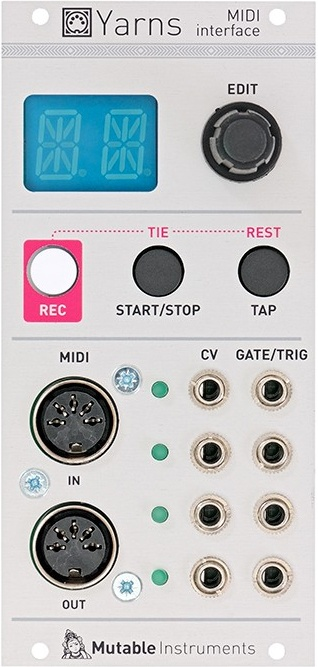
\includegraphics[width=0.2\textwidth]{graphics/yarns.jpg}
    \caption{\textit{Yarns} hardware sequencer by \textit{Mutable Instruments}. Source: 
    https://www.modulargrid.net/e/mutable-instruments-yarns}
    \label{fig:yarns}
\end{figure}
\subsubsection{Polyrhythmus}
\textit{Polyrhythmus} is a \textit{Max for Live} plugin for \textit{Ableton Live}. \textit{Max for Live} is visual programming language designed for audio synthesis and music composition. It is integrated into \textit{Ableton Live} allowing users to develop their own synthesizers or effects and use them directly in their music. \textit{Polyrhythmus} is an example of this and it features a user interface for programming 5 polyrhythmic sequences. It uses the euclidean algorithm to maximize onset evenness within a given number of bars, by changing the step time. This makes it a polyrhythmic sequencer, as opposed to the polymetric feature of traditional euclidean rhythms.\cref{sec:polyrhythmic}.\\
Programming Polyrhythmus involves, specifying each single step to be associated with an onset. In this way, it can generate the same rhythmic patterns as the euclidean framework, but in a very complicated way, that limits the possibility for quick changes.\\
The device features a linear graphical representation of the patterns, providing a nice overview of the progression, see \cref{fig:polyrhythmus}.

\begin{figure}[H]
    \centering
    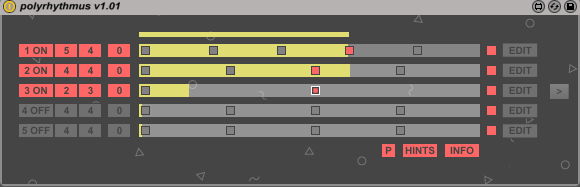
\includegraphics[width=\textwidth]{graphics/polyrhythmus.PNG}
    \caption{Screenshot from Ableton Live, showing the sequencer overview window of the polyrhythmus device. Yellow markers, shows progression for each rhythmic patterns. The 2 upper patterns represents the same polyrhythm, 5/4 , given in musical notation in \cref{fig:poly}}
    \label{fig:polyrhythmus}
\end{figure}

\section{Design requirements}
\label{sec:design_requirements}
The purpose of this project is to design a sequencer according to the following specifications, derived from the analysis above.

\noindent The sequencer:
\begin{enumerate}
    \item \label[req]{req:hardware} is implemented as hardware with a physical user interface
    \item \label[req]{req:playback}  has programmable playback only and no recording capabilities
    \item \label[req]{req:rhythm} is meant for programming rhythms (melodies are out of scope)
    \item \label[req]{req:communicate} communicates with software audio modules only
    \item \label[req]{req:time} has time resolution of 96 parts per quarter note
    \item \label[req]{req:euclid} generates musical events using euclidean rhythms with the following additions:
    \begin{enumerate}
        \item \label[req]{req:onset} possibility of rhythms with dynamic onset-density
        \item \label[req]{req:expressive} possibility of expressive timing
        \item \label[req]{req:velocity} possibility of dynamic accentuation 
    \end{enumerate}
    \item \label[req]{req:gui} features a graphical cyclic representation
\end{enumerate} 
  

